\documentclass[10pt,letterpaper]{article}
\usepackage{amsmath}
\usepackage{amsfonts}
\usepackage{amssymb}
\usepackage[english]{babel}
\usepackage{breakurl}
\usepackage[superscript]{cite}
\usepackage{draftwatermark}
\usepackage{fancyhdr}
\usepackage{float}
\usepackage[margin=1in]{geometry}
\usepackage{graphicx}
\usepackage{hyperref}
\usepackage[utf8]{inputenc}
\usepackage{makeidx}
\usepackage{multicol}
\usepackage{nth}
% \usepackage[default,scale=1.0]{opensans} % CHANGED:
\usepackage{setspace}
\usepackage{siunitx}
\usepackage{svg}
\usepackage{subcaption}
\usepackage{tikz}
\usepackage{url}

% [PREAMBLE]
% Custom commands
\newcommand{\ts}{\textsubscript}

% !!! Global variables
\newcommand{\titletext}{Exploration of Design Patterns in Game Development}

% New flags
\newif\iftwocolumns

% Set flags
\twocolumnsfalse

% Double spacing
% \doublespacing

% Watermark
\SetWatermarkText{Draft}
\SetWatermarkScale{5}
\SetWatermarkColor[gray]{0.95}

% Use hyphans to break up urls
\def\UrlBreaks{\do\/\do-}

% Hyper ref setup
\hypersetup{
	colorlinks=true,
	citecolor=black,
	linkcolor=black,
	filecolor=black,
	urlcolor=blue,
	pdftitle={APSC 310 Technical Report - Muchen He},
	bookmarks=true
}
\urlstyle{same}

% Page semantics
\pagestyle{fancy}

% Header
\fancyhead[L]{\MakeUppercase{APSC 310}}
\fancyhead[R]{Muchen He}
\fancyfoot{}
\fancyfoot[C]{\thepage}

% Page indent
\parindent 0ex

% Metadata
\author{Muchen He}
\title{APSC 310 Work Term Technical Report}

% [DOCUMENT]
\begin{document}

% [TITLE PAGE]
\begin{titlepage}
	\begin{center}
		\vspace*{3in}
		\line(1, 0){400}\\
		\Huge{\textbf{\titletext{}}}\\[0.2cm]
		\large{\textbf{Technical Work Term Report (Work Term 3)}}\\[1cm]
		\Large{\textbf{APSC 310}}\\
		\textbf{University of British Columbia}\\
		\line(1, 0){400}\\
		\vfill
		\Large{Muchen He}\\
		\large{Associate Developer, BioWare Edmonton}\\
		Student Number: 44638154\\

		\today \\
	\end{center}
\end{titlepage}

% [TOC]
\setcounter{secnumdepth}{3}
\tableofcontents
\thispagestyle{empty}
\clearpage

% [PREFACE]

% Set page numbering to roman for preface
\pagenumbering{roman}

% !!! Preface
\section*{Preface \& Foreword}
\addcontentsline{toc}{section}{Preface \& Foreword}

% Purpose
\subsection*{Purpose}
\addcontentsline{toc}{subsection}{Purpose}

The purpose of this report is to explore and observer different kinds of theoretical methods nad patterns and how they're used ot develop components that make up a game.\\
\\
As well to consolidate my knowledge as a whole in the industry as design patterns are software development concepts and potentially applicable elsewhere in the tech industry.

% Background
\subsection*{Background}
\addcontentsline{toc}{subsection}{Background}

(Working at EA-Bioware)
(Associate Developer (Programmer) for game Anthem)
(Using modern game engine Frostbite)

% Scope
\subsection*{Scope of Coverage}
\addcontentsline{toc}{subsection}{Scope of Coverage}

(The scope of this report)(Covers many design patterns outlined in ``Gang of Four'')(Will not cover detailed breakdown, explaination, and specification of existing proprietary tech; i.e. extended code from the game or Frostbite engine)

The technical coverage cited in this report is limited because the co-op work term position is working in UI/UX. Thus I lack understanding in other areas of the game such as character handling, world rendering, etc. Many of the workflows I describe in this report may only apply to UI/UX development within this project.

% (Other) Contributors
\subsection*{Contributors}
\addcontentsline{toc}{subsection}{Contributors}

(Tim Gibson - senior software lead, manager: contribution by supervising the report and giving advice) 

\newpage

% !!! [SUMMARY]
\section*{Summary}
\addcontentsline{toc}{section}{Summary}
\newpage

% [List of Figures/Tables]
% \thispagestyle{empty}
\listoffigures
\addcontentsline{toc}{section}{List of Figures}
\listoftables
\addcontentsline{toc}{section}{List of Tables}
\newpage

% Reset page counter
\pagenumbering{arabic}
\setcounter{page}{1}
\setcounter{section}{0}

% !!! [INTRODUCTION]
\iftwocolumns
\begin{multicols}{2}
\fi

% ??? [DISCUSSION]
\section{Introduction}

This enters the discussion portion of the report. We will analyze the current processes in game development for UI/UX at BioWare. Then look at some of the more theoretical, templated solutions known as design patterns in later sections and draw comparisons. We will also look into how the design patterns would be used in a general sense in game development (not specific to BioWare or Bioware's current project, Anthem).

\subsection{Game Development Overview}

% There are many parts to a video game. It can be grouped into: rendering, physics / simulation, AI, UI, sound / music. online, controls (input handling), online / networking. All tied together by the game engine.\\

% Having all the systems working together monolithically is bad, becuase it's difficult to maintain, prone to errors and bugs, and hard to collaborate as sub-systems are too tightly coupled.\\

% Talk about the video game industry -> video game development
% -> video game roles
A major portion of the video game market consists of AAA (Triple-A) video games. These are titles with very high production value, large budget, and typically consists of a team of hundreds of developers. These developers consist of artists, scripters, programmers, managers, etc. Many of these roles are further grouped into sub-teams such as rendering, physics/simulation, AI, UI/UX, sound design, music production, networking, etc. Individual developers are specialized to work on one part of the game, with the exception of leads, managers, and other executives.

\subsubsection{Game Engine}
Developers will use a game engine so that many people can work on the project at once. The game engine is generally highly optimized for graphics rendering, physics simulation (such as collision detection), and object handling.\\

The Frostbite engine is the game engine widely adoped at Electronic Arts (EA) studios. It was originally developed by Digital Illusions CE (DICE).\cite{frostbite}\cite{frostbite-wiki} As expected, the game engine is a piece of software, thus it is prone to software development problems that design patterns are ought to solve.

\subsection{Game Building}

Programmers make primitive entities such as an abstract UI widget, as well as the system that manages these entities.\\
\\
The scripters and artists then use these entities in \textit{schematics}, which are blocks of game content that contains logic and output, given some input.\\
\\
These schematics are in game levels, UI widgets, and prefabricated logic blocks (LogicPrefab). Thousands of these make up functionalities in a game, and are all handled by the game engine.


\subsubsection{Role of Programmers}

At BioWare, most game programmers work with code (in C++ and C\#). Programmers are specialized to develop in-game entities, or tools for scripters, designers, and artists. Programmers also integrate systems together, such as making mouse inputs interact with hitzones widgets, which interacts with graphical widgest or animation timelines.\footnote{Animation timelines are timeline that describe how a particular object will animate. Example: a fade in.}


\subsection{Design Pattern}

Design patterns are reusable, general, abstract solutions to common problems in software developent.\cite{sm-designpatterns} Design patterns are meant to be used when there no problems actually exist -- doing so would cause excess undesired complexity.

\subsubsection{Antipatterns}
Software written without care are difficult to maintain, prone to bugs and errors, and hard to collaborate. Software written with these ``hacks'' are known as \textit{antipatterns}, where there is more negative consequences than the benefits of its solution. Antipatterns are counter parts to correctly implemented design patterns.\cite{sm-antipatterns}\\
\\
Avoid antipatterns as much as possible. Exploring the negative effects of antipatterns is not part of the scope of this report.

\subsection{Gang of Four}

In software development, the phrase ``Gang of Four'' refers to the four authors of the Design Patterns book. The book features the most common design patterns widely in use today.\\


\section{Creational Design Patterns}

Creational design patterns involves with object creation.\cite{sm-creationaldp} This is especially useful in game development, such as when we need to create many trees or bushes in a level of a game. These patterns become more useful when the objects we're trying to create have relationships, such as \textit{inheritance}, to other objects.\\
\\

\subsection{Builder}

In object oriented programming, the construction of an instance of an object takes parameters. It is possible  that we need a lot of parameters to satisfy more variants of the class. This introduces the telescoping constructor antipattern\cite{telescopingconstructor}, where there are numerous variations of constructor methods all delegate to the default constructor. The problem is having this many constructor methods with slight variations is hard to maintain and difficult to use. When creating a new instance (invoking the constructor), it's hard to tell what the actual paramters are if they have the same type.\\
\\
The builder pattern encapsulates the parameters into a single structure. The structure itself is then passed into the constructor method, where we can access the data inside the structure again. The members of the structure can be accessed and modified by name, thereby eliminating the ambiguity of telescoping constructor.\\

This is useful in games. For example, a customizable character would have many parameters to be varied (Figure \ref{fig:playercharacter-1}).

\begin{figure}[H]
	\centering
	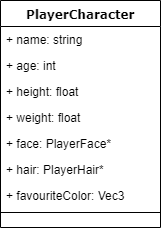
\includegraphics[scale=0.5]{assets/playercharacter_class}
	\caption{PlayerCharacter class with various desired parameters}
	\label{fig:playercharacter-1}
\end{figure}

\subsection{Factories}

\subsection{Object Pool}

\subsection{Prototype}

\subsection{Singleton}

In a way, they're just glorified global variable.


\section{Behaviour Design Patterns}

\section{Structural Design Patterns}

\section{Architectural Patterns}

\subsection{Entity-Component-System}

\subsubsection{Composition over Inheritance}

\subsection{Model-View-Controller}

Mostly used in UI development. 

% !!! [CONCLUSION]
\section{Conclusions}

\iftwocolumns
\end{multicols}
\fi

% !!! [BIBLIOGRAPHY]
\clearpage
\addcontentsline{toc}{section}{References}
% \bibliographystyle{apalike}
\bibliographystyle{ieeetr}
\bibliography{references}

% !!! [APPENDIX]
\clearpage
\appendix
\section{Sample Code}

% End of document
\end{document}